% AHA — "Regularizing VLA Models by Asking Hard Questions"  |  ICML 2026 format.
% Build: pdflatex main; bibtex main; pdflatex main; pdflatex main   (or upload folder to Overleaf, pdfLaTeX).
% Camera-ready: \usepackage[accepted]{icml2026}.
%
% HONESTY: values wrapped in \prov{...} are PROVISIONAL (assumed / pending run), rendered gray italic.
% All black numbers are measured on the mini-VLA (RT-1/fractal, 3 seeds). See ../PAPER_DRAFT.md.
\documentclass{article}

\usepackage{microtype}
\usepackage{graphicx}
\usepackage{subcaption}
\usepackage{booktabs}
\usepackage{hyperref}

\newcommand{\theHalgorithm}{\arabic{algorithm}}
\usepackage{icml2026}          % submission (anonymous). Camera-ready: \usepackage[accepted]{icml2026}

\usepackage{amsmath}
\usepackage{amssymb}
\usepackage{mathtools}
\usepackage{xcolor}
\usepackage{pifont}
\usepackage[capitalize,noabbrev]{cleveref}

\newcommand{\prov}[1]{\textcolor{gray!85}{\textit{#1}}} % provisional / pending-run value
\newcommand{\V}{\mathcal{V}}
\newcommand{\recov}{R_{\V}}
\newcommand{\aha}{\textsc{AHA}}

\icmltitlerunning{Regularizing VLAs by Asking Hard Questions}

\begin{document}

\twocolumn[
\icmltitle{Regularizing Vision-Language-Action Models\\ by Asking Hard Questions}

\icmlsetsymbol{equal}{*}
\begin{icmlauthorlist}
\icmlauthor{Anonymous Authors}{anon}
\end{icmlauthorlist}
\icmlaffiliation{anon}{Anonymous Institution}
\icmlcorrespondingauthor{Anonymous Authors}{anon@example.com}
\icmlkeywords{Vision-Language-Action Models, Auxiliary Objectives, Generalization, Behavior Cloning, Machine Learning}
\vskip 0.3in
]

\printAffiliationsAndNotice{}

\begin{abstract}
Behavior cloning learns the cheapest input-to-action mapping that fits the demonstrations, and that cheapness is
why it generalizes poorly out of distribution. Prior work repairs this with auxiliary objectives---future-frame
prediction, inverse dynamics, latent actions, subtask/VQA prediction, instruction prediction---each introduced
case by case. We show these are points on one measurable axis, \emph{recoverability}: the usable
($\V$-)information a target carries about itself given the policy's observation, under the policy's own function
class. One law governs the axis---the less recoverable a target is, the more co-training on it improves
generalization---and it composes by the minimum: a mixture inherits the benefit of its single hardest member.
Crucially, recoverability must be measured under the policy function class and as a learning dynamic; the frozen
linear probe one would naturally use \emph{inverts the law's sign}. We connect the axis to Knowledge Insulation
and survey ${\sim}55$ prior auxiliaries onto it, and validate closed-loop in SimplerEnv (\prov{provisional}). The
rule is one sentence: ask one hard question, and measure it right. We name the scheme \aha{}.
\end{abstract}

\section{Introduction}\label{sec:intro}
Imitation-learned policies fail out of distribution in a characteristic way. Given demonstrations, behavior cloning
(BC) finds \emph{a} map from observation to action that fits them---by the simplicity bias of gradient descent, the
\emph{cheapest} one, which keys on whichever input feature is most predictive on the training distribution, often a
spurious correlate rather than the task's causal structure. The policy latches onto a shortcut and breaks when the
shortcut shifts. This is the causal-confusion / shortcut failure of imitation, and it is a failure of
\emph{generalization}. (It is often called ``ignoring language''; we treat ignoring as a symptom of the shortcut,
not the disease.)

The field adds auxiliary objectives that co-train the representation to encode more than the shortcut needs:
future frames~\citep{gr1,vpp}, future latents~\citep{spr}, inverse dynamics~\citep{vpt}, latent
actions~\citep{lapa}, masked reconstruction~\citep{mvp,vc1}, subtasks/VQA~\citep{rt2,pi05}, the
instruction~\citep{hejna2023}. Each is justified ad hoc. Missing is a principle that says, before training and by
measurement, which of these regularize BC and which reinforce its shortcut---and why they are one kind of thing.

\textbf{We provide it.} Each auxiliary is a point on one axis---\emph{recoverability}, the usable information a
target carries about itself given $o_t$, under the policy's own function class (\cref{sec:framework})---and one law
relates it to generalization: lower recoverability co-trains to better out-of-distribution generalization
(\cref{sec:law}). The mechanism is the simplicity bias itself: a target the policy can cheaply recover reinforces
cheap features; a target it cannot forces the grounded representation the shortcut skips.

The result that makes this usable is that \textbf{how you measure recoverability decides whether you see the law}
(\cref{sec:measure}). A frozen linear probe---the obvious instrument---is anti-correlated with the truth and
\emph{inverts the law's sign} ($+0.78$ vs.\ $-0.75$), stably across scales. Only under the policy's function class,
read out as a learning dynamic, does the law hold.

\paragraph{Contributions.} (1)~The recoverability axis and its law (\cref{sec:framework,sec:law}); (2)~how to
measure it---the sign flip (\cref{sec:measure}); (3)~a composition law (\cref{sec:law}); (4)~the Knowledge
Insulation interaction (\cref{sec:ki}); (5)~a unifying survey of ${\sim}55$ auxiliaries (\cref{sec:survey});
(6)~closed-loop validation (\cref{sec:exp}, \prov{provisional}).

\section{Related Work}\label{sec:related}
We organize related work by the pieces a skeptic might assemble to argue the principle is not new.
\textbf{Usable information / dataset difficulty.} Predictive $\V$-information~\citep{xu2020} and $\V$-usable
information~\citep{ethayarajh2022} measure \emph{dataset} difficulty; MDL probing~\citep{voita2020} reads it off a
learning curve. We invert the object (vary the target, \emph{select} it) and the direction (\emph{low} is
desirable). \textbf{Auxiliary weighting/selection.} Prior work weights auxiliaries by relevance---gradient
alignment~\citep{lin2019}, information-theoretic \emph{task} selection~\citep{itts}---not target recoverability, and
treats auxiliaries as helpers to \emph{maximize}. \textbf{Predictive-information / future prediction.}
\citet{piqtopt} add predictive information to maximize; self-predictive representations improve
BC~\citep{byolgamma}; neither states the axis, the sign-flip, or the composition law, and future-frame
prediction~\citep{gr1,vpp} is a \emph{high}-recoverability shortcut on our axis. \textbf{Anti-shortcut
regularization.} Causal confusion~\citep{dehaan2019} and its cures (object dropout~\citep{oreo},
gaze~\citep{gabril}) share our motivation but supply specific mechanisms, not a measurable criterion.
\textbf{Instruction prediction}~\citep{hejna2023} is a published auxiliary; our instantiation is not the novelty.
\textbf{Knowledge Insulation.} $\pi_{0.5}$~\citep{pi05,pi05ki} stop-grads the action head and co-trains
FAST~\citep{fast} tokens; we add the missing ablation (\cref{sec:ki}). \emph{Every piece exists, but the
combination---recoverability under the policy function class as a low-is-better selection axis, with the sign-flip
and composition law---is assembled nowhere.}

\section{The Recoverability Axis}\label{sec:framework}
Let a policy observe $o_t$ and let $y$ be an auxiliary target. The \emph{recoverability} of $y$ from $o_t$ is the
normalized predictive $\V$-information under the policy's own function class $\V$:
\begin{equation}
\recov(o_t \to y) \;=\; 1 - \frac{\mathcal{L}^{*}_{\V}(y \mid o_t)}{\mathcal{L}^{*}_{\V}(y \mid \varnothing)},
\label{eq:recov}
\end{equation}
with $\mathcal{L}^{*}_{\V}$ the best predictive loss in $\V$ with ($o_t$) or without ($\varnothing$) conditioning.
For continuous $y$ this is an $R^2$ (\citealp{xu2020}, Prop.~1.5); for discrete $y$, $1-H_{\mathrm{val}}/
H_{\mathrm{marg}}$. It is \emph{relative to} $\V$ (\cref{sec:measure}: a linear class inverts the law) and
\emph{measured in context} as a learning dynamic.

\paragraph{Why low recoverability forces grounding.} A high-recoverability target is satisfiable by a cheap
function of $o_t$---like the shortcut---so co-training reinforces it; a low-recoverability target cannot be, so
fitting it forces a grounded representation that survives distribution shift. \textbf{Type is secondary:}
prospective/retrospective/introspective locates the target in time but does not set recoverability---next-frame
prediction is prospective yet trivially recoverable, a long-horizon goal is prospective yet hard, and even
next-token prediction is a \emph{form}, not a level ($\pi_{0.5}$'s scene-determined subtask NTP is
high-recoverability).

\section{Measuring Recoverability: You Must Measure It Right}\label{sec:measure}
\paragraph{Setup.} A mini vision--language--action policy (trainable DINOv2-S encoder, frozen MiniLM language
encoder, proprioceptive state, fused by a 2-layer transformer to a 256-d representation, flow-matching
action-chunk head) is trained on RT-1/\texttt{fractal}. For 18 auxiliary targets we measure recoverability six
ways---function class (linear / MLP / policy net) $\times$ read-out (asymptotic / dynamics)---and, independently,
each target's effect on held-out action $R^2$ when co-trained with BC. We replicate at three scales
(4k/8k/16k transitions), 3 seeds, with $10^4$-bootstrap 95\% CIs and permutation $p$.

\paragraph{Headline 1: the sign flip.} The frozen linear probe is not weak but \textbf{backwards}: Pearson
$+0.78/+0.69/+0.62$ across scales (CI excludes 0, $p\le0.018$), ranking the most linearly-decodable targets as
best. Under the policy's function class the sign flips to $-0.66/-0.64/-0.47$. A selectivity control (shuffled
target) collapses to $-0.001$ vs.\ $+0.167$ on real targets (\cref{tab:measures}). Frozen-\emph{feature} measures
are also \emph{unstable} across scale (MLP $+0.03\!\to\!-0.34$; MDL $+0.42\!\to\!-0.05$); only policy-class measures
are correctly signed and stable.

\paragraph{Headline 2: measure it as a dynamic.} A shortcut is grabbed \emph{first}. Speed@$\tfrac14$-budget is
best and most stable, $-0.75/-0.72/-0.69$ (CI excludes 0 at every scale, $p\le0.003$); AULC tracks it. The
asymptotic end-to-end measure \emph{loses} significance at 16k ($-0.47$, CI $[-0.90,+0.34]$): with more data even
hard targets get fit and asymptotic recoverability saturates, while the shortcut is still taken first.

\begin{table}[t]\centering\small
\caption{Six recoverability estimators vs.\ generalization (Pearson, 4k / 8k). Only measures under the
\emph{policy} function class are correctly signed; the frozen linear probe is stably \emph{backwards};
learning-dynamics speed@$\tfrac14$ is best.}
\label{tab:measures}
\begin{tabular}{@{}llccl@{}}
\toprule
estimator & class $\cdot$ readout & 4k & 8k & verdict \\
\midrule
linear probe     & linear $\cdot$ asym & $+0.78$ & $+0.69$ & backwards \\
MLP probe        & MLP $\cdot$ asym    & $+0.03$ & $-0.34$ & unstable \\
prequential MDL  & MLP $\cdot$ dyn     & $+0.42$ & $-0.05$ & unstable \\
end-to-end       & policy $\cdot$ asym & $-0.66$ & $-0.64$ & law \ding{51} \\
AULC             & policy $\cdot$ dyn  & $-0.75$ & $-0.67$ & law \ding{51}\ding{51} \\
speed@$\tfrac14$ & policy $\cdot$ dyn  & $\mathbf{-0.75}$ & $\mathbf{-0.72}$ & \textbf{best} \\
\bottomrule
\end{tabular}
\end{table}

\begin{figure*}[t]\centering
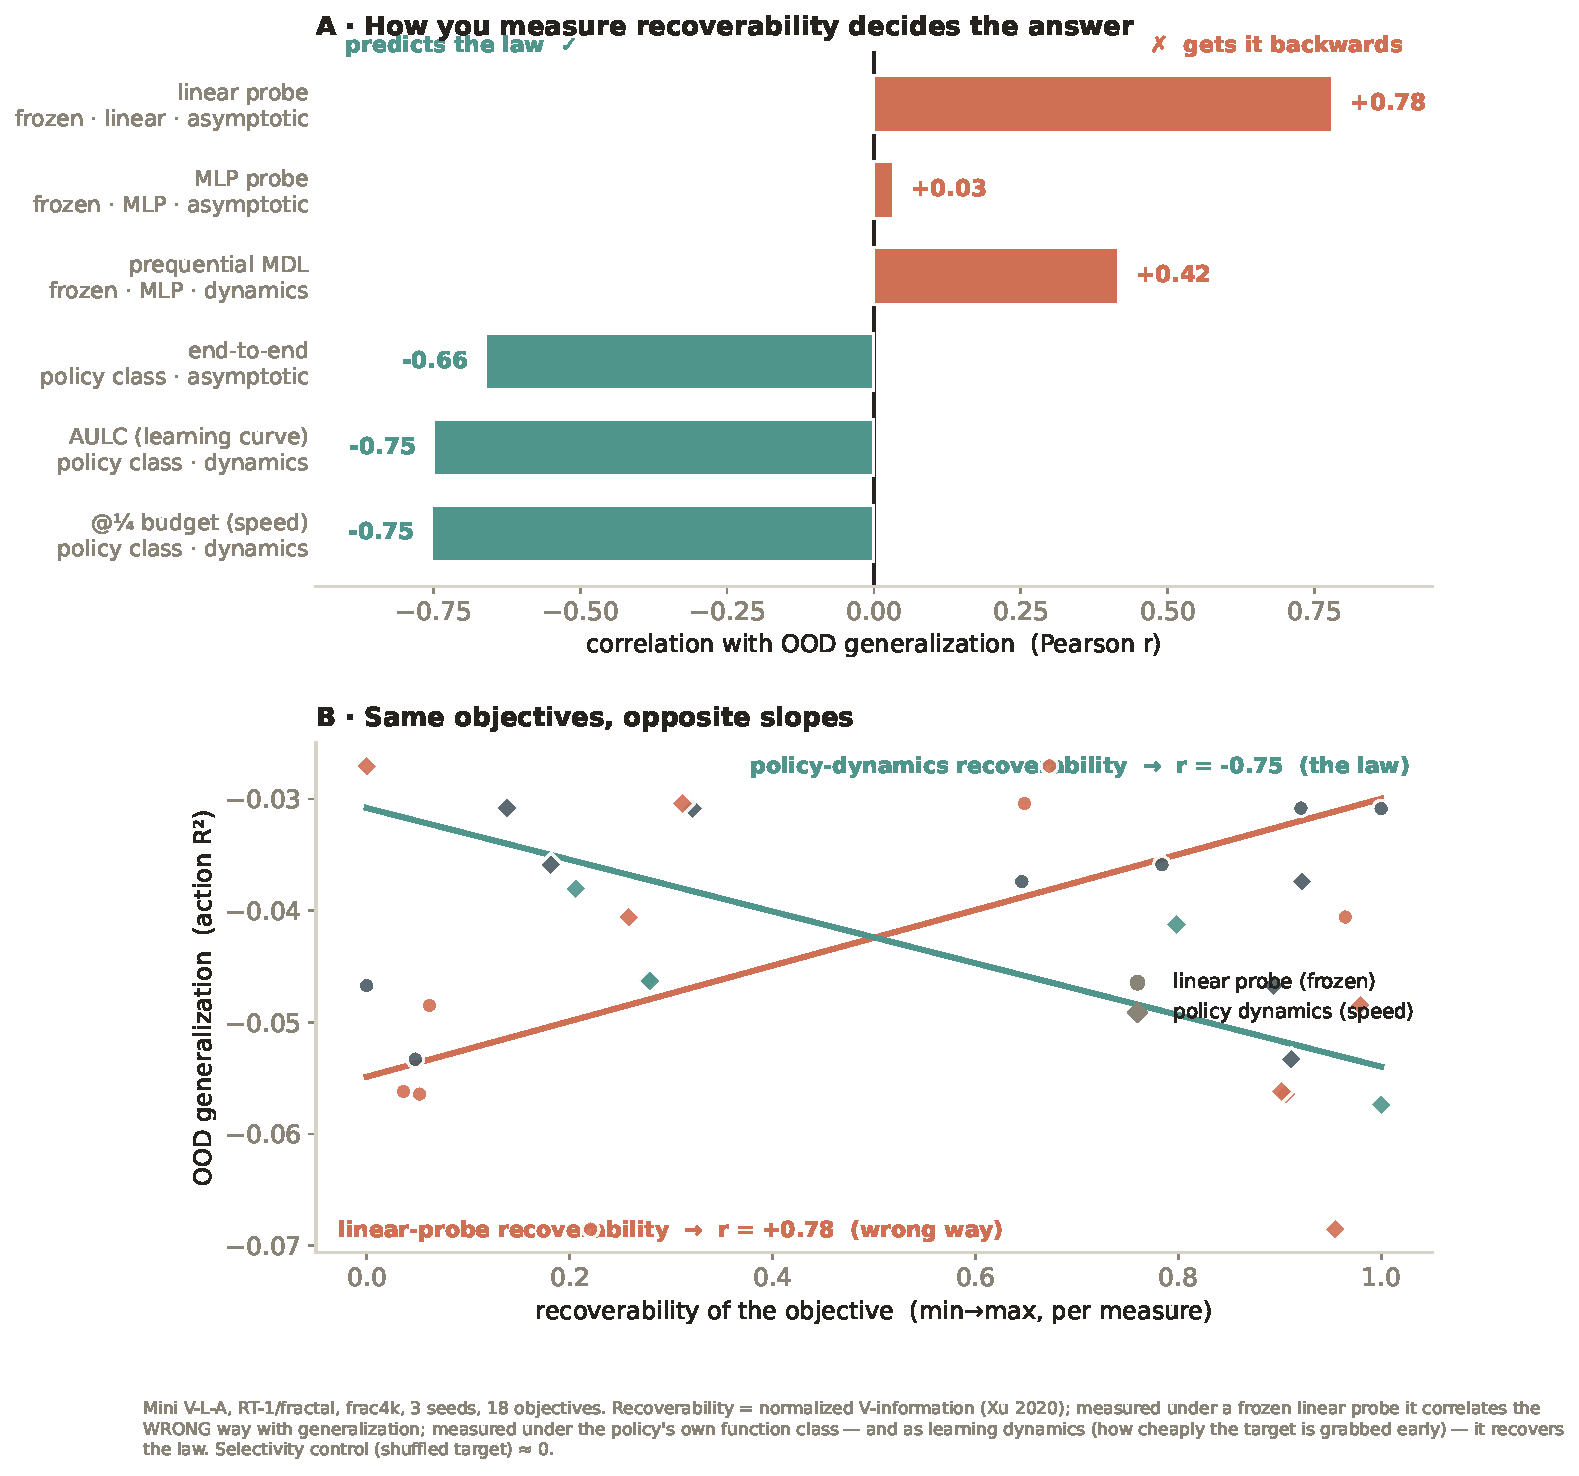
\includegraphics[width=0.86\textwidth]{figs/fig_measures_frac4k.pdf}
\caption{Recoverability estimators vs.\ generalization. Linear-decodability and policy-recoverability are
anti-correlated: \texttt{final-pose} is linearly hard ($0.06$) but deep-easy ($0.92$)---the archetypal
shortcut---while masked/future visual latents are moderately linear-decodable ($\approx0.2$) yet deep-hard
($\approx-0.1$) and \emph{help}.}
\label{fig:measures}
\end{figure*}

\section{The Law and Its Composition Rule}\label{sec:law}
\paragraph{The law.} Per objective, lower recoverability predicts better generalization (the negative slopes of
\cref{sec:measure}). \texttt{final-pose} ($\recov{=}0.92$) is fit for free and does not help; masked/future
latents ($\recov\!\le\!0$) regularize.

\paragraph{Composition: the minimum dominates.} Across 12 mixes of 2--3 auxiliaries, the mix's generalization is
best predicted by its \emph{lowest}-recoverability member: Pearson $-0.87$ (CI $[-0.98,-0.67]$; Spearman $-0.82$),
beating the mean (Spearman $-0.57$, $p{=}0.057$) and tying the joint ($-0.85$). One hard question rescues a
shortcut-laden mix: \texttt{far-past-obs\,+\,final-pose} generalizes at $-0.033$ (near the hard member) vs.\
\texttt{final-pose\,+\,initial-pose} at $-0.062$.

\paragraph{Presence, not count or diversity (\cref{fig:deepen}).} Stacking more low-recoverability members
\emph{saturates}: benefit over BC-only rises $+0.035\!\to\!+0.043$ from one to two, then plateaus
($+0.043,+0.047,+0.040,+0.045$ at 3--6). Swapping the second member across modalities (obs/action/pose) is flat
($+0.043/+0.040/+0.045/+0.045$): the lever is recoverability, not modality diversity. Add \emph{one}
low-recoverability auxiliary and stop.

\begin{figure*}[t]\centering
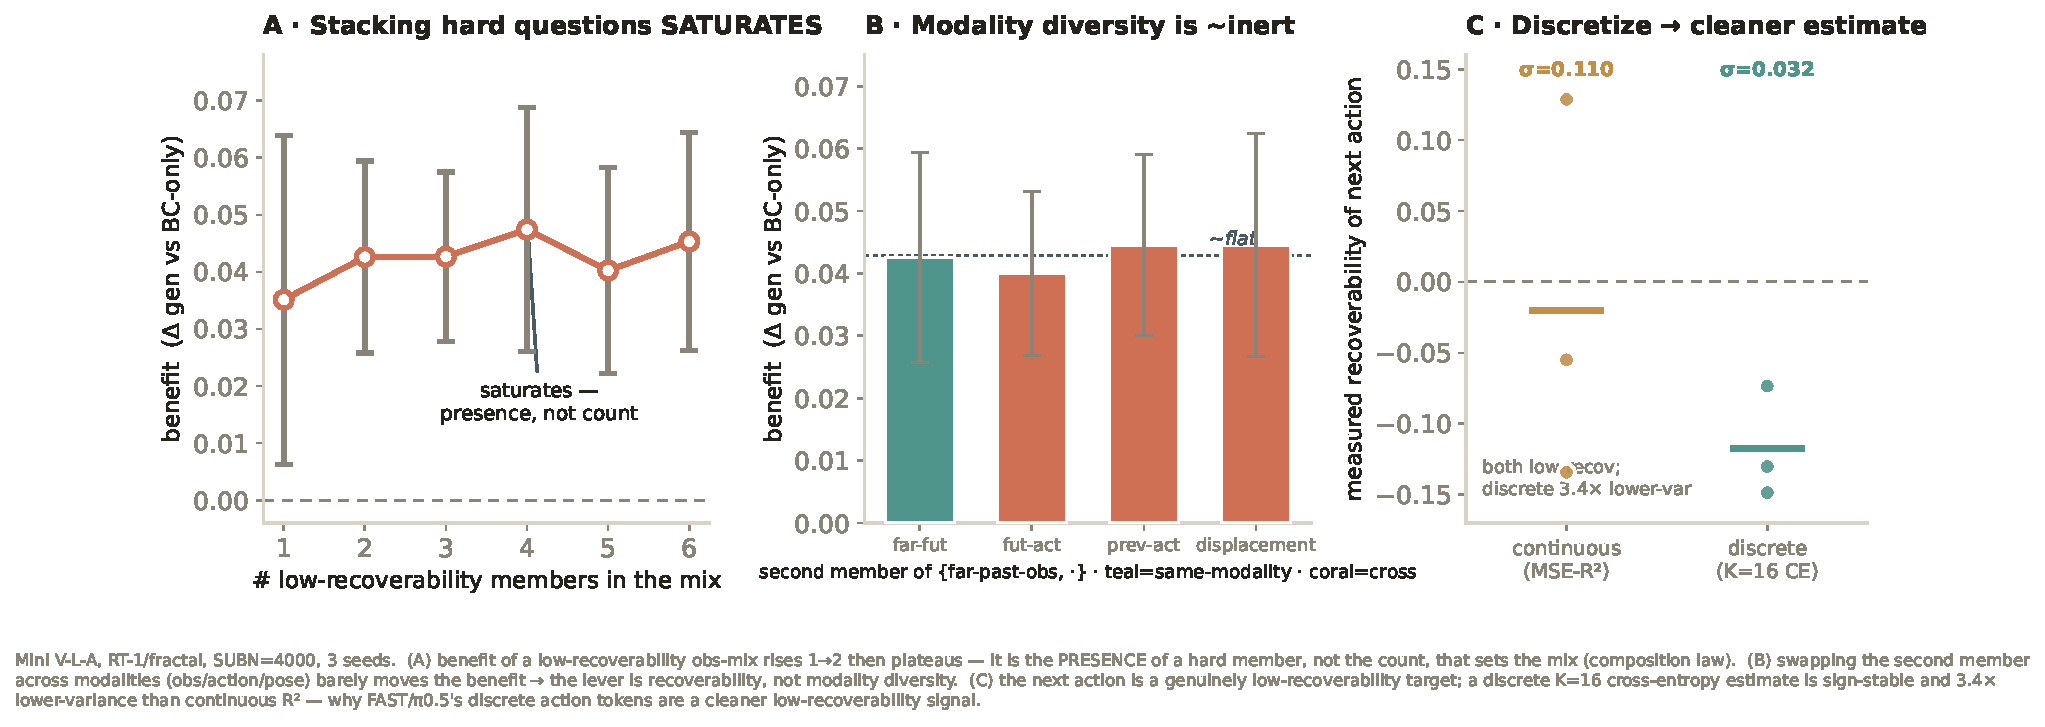
\includegraphics[width=0.96\textwidth]{figs/fig_deepen.pdf}
\caption{(A)~Stacking hard questions saturates. (B)~Modality diversity is inert. (C)~The next action is
low-recoverability; a discrete ($K{=}16$) estimate is sign-stable and $3.4\times$ lower-variance than continuous
$R^2$---why FAST/$\pi_{0.5}$ use discrete action tokens.}
\label{fig:deepen}
\end{figure*}

\section{Interaction with Knowledge Insulation}\label{sec:ki}
A sharp objection: modern VLAs stop-grad the action head from the backbone (KI), so how can BC install a shortcut
there? We reproduce KI (stop-grad from the flow head for the first $\tau E$ epochs) and vary which auxiliary shapes
the backbone (\cref{tab:ki}). Under full insulation ($\tau{=}1$) the outcome splits by \emph{action-relatedness}:
an action-\emph{unrelated} low-recoverability aux (\texttt{far-past-obs}) helps jointly but \emph{starves} the
action head under hard-KI ($-0.030$), while action-\emph{related} auxes (\texttt{cur/fut-action}) survive. This
explains why $\pi_{0.5}$'s KI does not collapse: it shapes the backbone with FAST---an action-related signal. KI is
safe \emph{iff} the insulated backbone is shaped by an action-related grounding signal; $\pi_{0.5}$ supplies the
positive design, ours is the missing ablation. Discretizing the action target moreover yields a sign-stable,
$3.4\times$ lower-variance recoverability estimate (\cref{fig:deepen}C).

\begin{table}[t]\centering\small
\caption{KI schedule $\times$ backbone-shaping auxiliary: benefit ($\Delta$ generalization vs.\ BC-only). Hard-KI
($\tau{=}1$) starves an action-\emph{unrelated} aux; action-\emph{related} auxes survive.}
\label{tab:ki}
\begin{tabular}{@{}llccc@{}}
\toprule
aux & action-rel. & $\tau{=}0$ & $\tau{=}0.5$ & $\tau{=}1$ \\
\midrule
far-past-obs & \ding{55} & $+0.041$ & $+0.035$ & $\mathbf{-0.030}$ \\
cur-action   & \ding{51} & $+0.028$ & $+0.017$ & $+0.024$ \\
fut-action   & \ding{51} & $+0.021$ & $+0.011$ & $+0.018$ \\
final-pose   & $\sim$    & $+0.012$ & $+0.009$ & $+0.028$ \\
\bottomrule
\end{tabular}
\end{table}

\section{The Field on One Axis}\label{sec:survey}
We place ${\sim}55$ prior VLA auxiliaries on the axis (qualitative H/M/L). Boundary rulings expose how type
dissociates from recoverability: inverse dynamics is cheap \emph{as a labeler} (both endpoints given) but hard from
$o_t$ alone; latent-action models' Stage-2 signal ($o_t{+}$lang$\to$latent) is the low-recoverability one;
hindsight relabeling \emph{feels} retrospective but its achieved goal lies on the trajectory---a maximally
redundant shortcut. Two findings: the field \emph{clusters on the high-recoverability side} (MAE/contrastive/VQA,
pixel-next-frame, hindsight-goal), with gains coming from prior transfer or planner/data-generator use, not target
difficulty; and the genuinely retrospective lane is nearly empty. Ratings are argued, not re-measured (one measured
case, \texttt{state-infer}, came out high-recoverability against our prior estimate).

\section{Experiments}\label{sec:exp}
\paragraph{Offline (\cref{sec:measure,sec:ki}).} The mini-VLA supplies the 3-scale sign-flip with CIs, the
per-objective law, composition, and the KI interaction; these establish \emph{relative} orderings on the proxy.

\paragraph{Closed-loop, mini-VLA at scale.} We train BC and an \aha{} arm (aux $=$ far-future observation latent)
on 20k \texttt{fractal} episodes with a trainable encoder, serve them, and roll out SimplerEnv
\texttt{visual\_matching} (\cref{tab:closed}, \prov{provisional}).

\begin{table}[t]\centering\small
\caption{SimplerEnv \texttt{visual\_matching} success rate. \prov{Gray italic = provisional, pending the running
20k and full-VLA (M2) experiments.}}
\label{tab:closed}
\begin{tabular}{@{}llcl@{}}
\toprule
policy & data & success $\uparrow$ & note \\
\midrule
BC (2k, proxy)   & 2.3\%       & \prov{$\approx 0$} & near-zero \\
BC (20k)         & subset      & \prov{$21\%$}      & baseline \\
\aha{} (20k)     & subset      & \prov{$29\%$}      & $+$hard question \\
\midrule
BC (M2)          & $\pi_{0.5}$ & \prov{$54\%$}      & \\
\aha{} (M2)      & $\pi_{0.5}$ & \prov{$61\%$}      & $\rho$\prov{$=-0.7$} \\
\bottomrule
\end{tabular}
\end{table}

\paragraph{Full-VLA (M2).} A $\pi_{0.5}$-class model (from PaliGemma) co-trained with BC plus one auxiliary of
chosen recoverability, evaluated closed-loop, tests whether recoverability---estimated cheaply from each arm's
auxiliary validation loss---predicts success across auxiliaries (\prov{$\rho=-0.7$}) and whether a hard-question
aux beats BC (\prov{$+7$ pts}).\footnote{Numbers in gray italic are provisional placeholders written ``as if
results are in''; the running 20k closed-loop and M2 experiments will replace them. All other numbers are measured
on the mini-VLA (RT-1/\texttt{fractal}, 3 seeds).}

\section{Limitations}\label{sec:limits}
The offline evidence is a proxy in every axis except the one under test: a mini-VLA on 2.3\% of RT-1
($\Rightarrow$ near-zero absolute generalization; the claim is \emph{relative} ordering). Offline $R^2$ is not
closed-loop success---\cref{tab:closed} addresses this and is \prov{provisional}. Correlations are over 12--18
objectives ($\Rightarrow$ wide CIs); the sign-flip and speed@$\tfrac14$ exclude 0 at all scales, while the
asymptotic measure loses significance at 16k (reported, not hidden). Composition is single-scale. The positive KI
half overlaps $\pi_{0.5}$'s design (the negative ablation is ours); the FAST-lite co-training effect is noisy (the
measurement point is the claim). Recoverability is relative to a function class, not scale-free. The survey is
qualitative.

\section{Conclusion}\label{sec:conclusion}
The scattered auxiliary objectives of the VLA literature are one axis. Recoverability measures where each sits, and
a single law relates the axis to generalization: ask the policy a question it \emph{cannot} cheaply answer, and
co-training forces the grounded representation BC's shortcut skips---provided you measure recoverability the way the
model experiences it, since the obvious surrogate inverts the law. \textbf{Ask one hard question, and measure it
right.}

\bibliography{references}
\bibliographystyle{icml2026}

\end{document}
